% The generic preamble
\documentclass[10pt,letterpaper,fleqn,titlepage]{article}

% Define packages to use
\usepackage{natbib}
\usepackage[dvips]{graphicx,color}
\usepackage{amsmath,amssymb}
\usepackage{bm}
\usepackage{caption}
\usepackage{xr}
\usepackage{ifthen}
\usepackage[dvipdfm,colorlinks,linkcolor=blue,citecolor=blue,urlcolor=blue]{hyperref}
\usepackage{fancybox}
\usepackage{textcomp}
\usepackage{alltt}
%\usepackage{floatflt}
%\usepackage{svn}


% Redefine default page
\setlength{\textheight}{9in}  % 1" above and below
\setlength{\textwidth}{6.75in}   % 0.5" left and right
\setlength{\oddsidemargin}{-0.25in}

% Redefine default paragraph
\setlength{\parindent}{0pt}
\setlength{\parskip}{1ex plus 0.5ex minus 0.2ex}

% Define caption width and default fonts
\setlength{\captionmargin}{0.5in}
\renewcommand{\captionfont}{\sffamily}
\renewcommand{\captionlabelfont}{\bfseries\sffamily}

% Define commands for super- and subscript in text mode
\newcommand{\superscript}[1]{\ensuremath{^\textrm{#1}}}
\newcommand{\subscript}[1]{\ensuremath{_\textrm{#1}}}

% Derived commands
\newcommand{\invcm}{\textrm{cm\superscript{-1}}}
\newcommand{\micron}{\ensuremath{\mu\textrm{m}}}

\newcommand{\df}{\ensuremath{\delta f}}
\newcommand{\Df}{\ensuremath{\Delta f}}
\newcommand{\dx}{\ensuremath{\delta x}}
\newcommand{\Dx}{\ensuremath{X_{max}}}
\newcommand{\Xeff}{\ensuremath{X_{eff}}}

\newcommand{\water}{\textrm{H\subscript{2}O}}
\newcommand{\carbondioxide}{\textrm{CO\subscript{2}}}
\newcommand{\ozone}{\textrm{O\subscript{3}}}

\newcommand{\taup}[1]{\ensuremath{\tau_{#1}}}
\newcommand{\efftaup}[1]{\ensuremath{\tau_{#1}^{*}}}

\newcommand{\textbfm}[1]{\boldmath\ensuremath{#1}\unboldmath}

\newcommand{\rb}[1]{\raisebox{1.5ex}[0pt]{#1}}

\newcommand{\f}[1]{\texttt{#1}}

% Define how equations are numbered
\numberwithin{equation}{section}
\numberwithin{figure}{section}
\numberwithin{table}{section}

% Define a command for title page author email footnote
\newcommand{\email}[1]
{%
  \renewcommand{\thefootnote}{\alph{footnote}}%
  \footnote{#1}
  \renewcommand{\thefootnote}{\arabic{footnote}}
}

% Define a command to print the Office Note subheading
\newcommand{\notesubheading}[1]
{%
  \ifthenelse{\equal{#1}{}}{}
  { {\Large\bfseries Office Note #1\par}%
    {\scriptsize \sc This is an unreviewed manuscript, primarily intended for informal}\\ 
    {\scriptsize \sc exchange of information among JCSDA researchers\par}%
  }
}

% Redefine the maketitle macro
\makeatletter
\def\docseries#1{\def\@docseries{#1}}
\def\docnumber#1{\def\@docnumber{#1}}
\renewcommand{\maketitle}
{%
  \thispagestyle{empty}
  \vspace*{1in}
  \begin{center}%
     \sffamily
     {\huge\bfseries Joint Center for Satellite Data Assimilation\par}%
     \notesubheading{\@docnumber}
  \end{center}
  \begin{flushleft}%
     \sffamily
     \vspace*{0.5in}
     {\Large\bfseries\ifthenelse{\equal{\@docseries}{}}{}{\@docseries: }\@title\par}%
     \medskip
     {\large\@author\par}%
     \medskip
     {\large\@date\par}%
     \bigskip\hrule\vspace*{2pc}%
  \end{flushleft}%
  \newpage
  \setcounter{footnote}{0}
}
\makeatother
\docseries{}
\docnumber{}


% Define a command for a DRAFT watermark
\usepackage{eso-pic}
\newcommand{\draftwatermark}
{
  \AddToShipoutPicture{%
    \definecolor{lightgray}{gray}{.85}
    \setlength{\unitlength}{1in}
    \put(2.5,3.5){%
      \rotatebox{45}{%
        \resizebox{4in}{1in}{%
          \textsf{\textcolor{lightgray}{DRAFT}}
        }
      }
    }
  }
}





%\includeonly{Introduction,Infrared_Channel_SRFs,Radiometric_Impact_of_Interpolation,Impact_of_Wide_Wings,srf.app,bc.app}
\includeonly{Introduction,srf.app,dtb.app}

% Definitions for tables
\newcommand{\frequency}[1]{\ensuremath{f_{#1}}}
\newcommand{\bfrequency}[1]{\boldmath\frequency{#1}\unboldmath}
\newcommand{\bdf}[1]{\boldmath\df{#1}\unboldmath}
\newcommand{\sideband}[1]{\ensuremath{df_{#1}}}
\newcommand{\bsideband}[1]{\boldmath\sideband{#1}\unboldmath}
\newcommand{\bdeltaf}{\boldmath\ensuremath{\Delta f}\unboldmath}
\newcommand{\up}[1]{\superscript{#1}}

% Title info
\title{ATMS NPP Spectral Response Function Analysis}
\author{P. van Delst\email{paul.vandelst@noaa.gov},
        D.N. Groff\email{david.groff@noaa.gov}\\JCSDA/EMC/SAIC\\[0.25in]
        W.J. Blackwell\email{wjb@mit.edu}\\Massachusetts Institute of Technology\\[0.25in]
        C.L. Chidester\email{Lynn.Chidester@sdl.usu.edu}\\Space Dynamics Laboratory, Utah State University\\[0.25in]
        G. De Amici\email{giovanni.deamici@ngc.com}\\Northrop Grumman Aerospace Systems\\[0.25in]
        S. Swadley\email{steve.swadley@nrlmry.navy.mil}\\Naval Research Laboratory}
\date{July, 2009}
\docnumber{(unassigned)}
\docseries{CRTM}


%-------------------------------------------------------------------------------
%                            Ze document begins...
%-------------------------------------------------------------------------------
\begin{document}
\maketitle

\draftwatermark

% The front matter
%=================
\thispagestyle{empty}
\vspace*{10cm}
\begin{center}
  {\sffamily\Large\bfseries Change History}
  \begin{table}[htp]
    \centering
    \begin{tabular}{|p{2cm}|p{3cm}|p{8cm}|}
      \hline
      \sffamily\textbf{Date} & \sffamily\textbf{Author} & \sffamily\textbf{Change}\\
      \hline\hline
      2009-07-01 & P. van Delst & Initial release.\\
      \hline
      2009-07-09 & P. van Delst & Added appendix B.\\
      \hline
    \end{tabular}
  \end{table}
\end{center}
\clearpage
\pagenumbering{arabic}
\setcounter{page}{1}


% The main matter
%================
\chapter{Introduction}
%=====================


\section{Components}
%===================
\label{sec:components}

The LBLRTM I/O library is constructed around five data constructs, described in table \ref{tab:component_definitions}:
\begin{table}[htp]
  \centering
  \caption{The data constructs of the LBLRTM I/O library}
  \begin{tabular}{p{2.5cm} p{12cm}}
    \hline\\[-0.1cm]
    \sffamily\textbf{Component Name} & \sffamily\textbf{Description} \\
    \hline\hline\\[-0.2cm]
    \texttt{Fhdr}  & The file header construct that is present at the start of each layer of data. \\\\
    \texttt{Phdr}  & This is the panel header construct that is present at the start of each ``chunk'' of data (usually referred to as a ``panel''. See following.) \\\\
    \texttt{Panel} & This construct corresponds to a ``chunk'' of spectral data. An LBLRTM datafile is referred to as being a single- or double-panel file. The former means a single spectral quantity is present (e.g. optical depth), and the latter means that two spectral quantities are present (e.g. radiance and transmittances). \\\\
    \texttt{Layer} & This construct contains spectral data for the entire frequency range of an LBLRTM calculation for a single layer. The concept ``layer'' can correspond to the spectral data for individual atmospheric layers of the input profile, or to the final result for an entire atmosphere. \\\\
    \texttt{File}  & This contruct is true to its name. It corresponds to an entire datafile of data which may consist of a single layer or multiple layers, and for single- or double-panel spectral data. \\
  \hline
  \end{tabular}
  \label{tab:component_definitions}
\end{table}

Each component has a definition module to define the object and some basic methods to manipulate it, and an I/O module to read and write instances of the objects from/to file.

Two components -- the file header and panel header -- are standalone, but the others contain other components, i.e. the panel object contains panel headers; the layer object contains file headers; and the file object contains layers. A schematic illustration of how the actual LBLRTM datafile format relates to the component definitions is shown in figure \ref{fig:lblrtm_format}.

Note, however, that when an LBLRTM file is read, the individual panel ``chunks'' of spectral data are concatenated into a single spectrum. Thus the \Panel{} object itself is only used when reading from an LBLRTM file and is not used in the \File{} or \Layer{} objects.

\begin{figure}[htp]
  \centering
  \input{graphics/lblrtm_format.pstex_t}
  \caption{Schematic illustration of the LBLRTM single- and double-panel datafile format. A datafile can contain one, or multiple, layers of data.}
  \label{fig:lblrtm_format}
\end{figure}



\section{Conventions}
%====================
\label{sec:conventions}
The following are conventions that have been adhered to in the current release of the LBLRTM I/O library. They are guidelines intended to make understanding the code at a glance easier, to provide a recognisable ``look and feel'', and to minimise name space clashes.



\subsection{Naming of Objects and Instances of Objects}
%------------------------------------------------------

The object\footnote{The terms ``derived type'' and ``structure'' can also be used as the code is not yet fully OO - that's for future updates.} naming convention adopted for use in the LBLRTM I/O library is, 

\hspace{0.4cm}\f{LBLRTM\_}\textit{name}\f{\_type} 

where \textit{name} is an identifier for the particular component (e.g. panel header, layer, file, etc as listed in table \ref{tab:component_definitions}). All object type names are suffixed with ``\f{\_type}''. The ``\f{LBLRTM\_}'' prefix is to define a namespace to minimise name clashes. An instance of a object is then referred to via its \textit{name}, or some sort of derivate of its \textit{name}. Some object declarations examples are,

\begin{alltt}
  TYPE(\hyperref[fig:LBLRTM_File_type_structure]{LBLRTM_File_type}) :: sp_file, dp_file
  TYPE(\hyperref[fig:LBLRTM_Layer_type_structure]{LBLRTM_Layer_type}) :: layer\end{alltt}



\subsection{Naming of Definition Modules}
%----------------------------------------

Modules containing object definitions are termed \textit{definition modules}. These modules contain the actual object definitions as well as various utility procedures that operate on the object. The naming convention adopted for definition modules in the LBLRTM I/O library is, 

\hspace{0.4cm}\f{LBLRTM\_}\textit{name}\f{\_Define} 

where all definition module names are suffixed with ``\f{\_Define}''. The actual source code files for these modules have the same name with a ``\f{.f90}'' suffix.



\subsection{Naming of I/O Modules}
%---------------------------------

Modules containing all the object I/O procedures are termed, surprise, surprise, \textit{I/O modules}. These modules contain function to read and write LBLRTM format datafiles. The naming convention adopted for I/O modules in the LBLRTM I/O library is, 

\hspace{0.4cm}\f{LBLRTM\_}\textit{name}\f{\_IO} 

where all I/O module names are suffixed with ``\f{\_IO}''. As with the definition modules, the actual source code files for these modules have the same name with a ``\f{.f90}'' suffix.



\subsection{Standard Definition Module Procedures}
%-------------------------------------------------

The definition modules for the user-accessible objects (for practical purposes just \File, although \Layer, \Fhdr, \Panel, and \Phdr are accessible for now) contain a standard set of procedures for use with the object being defined. The naming convention for these procedures is,

\hspace{0.4cm}\f{LBLRTM\_}\textit{name}\f{\_}\textit{action}

where the available default actions for each procedure are listed in table \ref{tab:definition_module_default_procedures}. This is not an exhaustive list but procedures for the actions listed in table \ref{tab:definition_module_default_procedures} are generally going to be present.

The exception is that the objects with no allocatable components do not have a creation procedure.

\begin{table}[htp]
  \centering
  \caption{Default action procedures available in object definition modules. $^{\dagger}$Procedures not available for the \Fhdr{} and \Phdr{} objects. $^{\ddagger}$Procedure available only for the \Layer{} object.}
  \begin{tabular}{p{2.5cm} p{3.5cm} p{8.5cm}}
    \hline\\[-0.1cm]
    \sffamily\textbf{Action} & \sffamily\textbf{Type} & \sffamily\textbf{Description} \\
    \hline\hline\\[-0.2cm]
    \texttt{OPERATOR(==)}             & Elemental function   & Tests the equality of two structures. \\
    \texttt{OPERATOR(/=)}             & Elemental function   & Tests the inequality of two structures. \\
    \texttt{Associated}$^{\dagger}$   & Elemental function   & Tests if the object components have been allocated. \\
    \texttt{Create}$^{\dagger}$       & Elemental subroutine & Allocates any allocatable object components. \\
    \texttt{Destroy}                  & Elemental subroutine & Reinitialises an object. \\
    \texttt{DefineVersion}            & Subroutine           & Returns the module version information. \\
    \texttt{Frequency}$^{\ddagger}$   & Subroutine           & Compute and return the spectral frequency grid. \\
    \texttt{Inspect}                  & Subroutine           & Displays object contents to \texttt{stdout}. \\
    \texttt{IsValid}                  & Elemental function   & Tests if the object contains valid data. \\
    \texttt{SetValid}                 & Elemental subroutine & Flags the object as containing valid data. \\
  \hline
  \end{tabular}
  \label{tab:definition_module_default_procedures}
\end{table}

\begin{table}[htp]
  \centering
  \caption{Default action procedures available in object I/O modules.}
  \begin{tabular}{p{2.5cm} p{3.5cm} p{8.5cm}}
    \hline\\[-0.1cm]
    \sffamily\textbf{Action} & \sffamily\textbf{Type} & \sffamily\textbf{Description} \\
    \hline\hline\\[-0.2cm]
    \texttt{IOVersion} & Subroutine  & Returns the module version information. \\
    \texttt{Read}      & Function    & Loads an instance of an object with data read from file. \\
    \texttt{Write}     & Function    & Write an instance of an object to file. \\
  \hline
  \end{tabular}
  \label{tab:io_module_default_procedures}
\end{table}

Some examples of these procedure names are,

\begin{alltt}
  \hyperref[sec:LBLRTM_File_Associated_interface]{LBLRTM_File_Associated}
  \hyperref[sec:LBLRTM_File_IsValid_interface]{LBLRTM_File_IsValid}
  \hyperref[sec:LBLRTM_Layer_Destroy_interface]{LBLRTM_Layer_Destroy}
  \hyperref[sec:LBLRTM_Layer_Frequency_interface]{LBLRTM_Layer_Frequency}
  \hyperref[sec:LBLRTM_File_Inspect_interface]{LBLRTM_File_Inspect}\end{alltt}

The relational operators, \f{==} and \f{/=}, are implemented via overloaded \f{Equal} and \f{NotEqual} action procedures respectively, as is shown below for the \File{} structure,

\begin{alltt}
  INTERFACE OPERATOR(==)
    MODULE PROCEDURE LBLRTM_File_Equal
  END INTERFACE OPERATOR(==)

  INTERFACE OPERATOR(/=)
    MODULE PROCEDURE LBLRTM_File_NotEqual
  END INTERFACE OPERATOR(/=)\end{alltt}

For a complete list of the definition and I/O module procedures for use with the available objects, see appendix \ref{app:object_and_interface_definition}.




\section{ATMS Response Data}
%===========================

\subsection{Specified and measured responses}
%--------------------------------------------
The NPP ATMS specified central frequencies, sideband offsets and channel bandwidths, taken from table 9 of reference \cite{CrIS_EDR_ATBD}, are shown in table \ref{tab:atms_fo_sb_and_df}. Also shown are measured bandwidths taken from table 12-1 of reference \cite{ATMS_PFM_CalLog}. No measurements of the central frequencies are readily available \footnote{These values may be available in other ATMS reports, particularly: RE-13680 K/Ka Band Receiver Shelf Verification Report, RE-13658 W Band Receiver Shelf Verification Report, RE-13741 V Band Receiver Shelf Verification Report, and RE-13802 G Band Receiver Shelf Verification Report.}.

\begin{table}[htp]
  \centering
  \begin{tabular}{c c c c c c}
    \hline
                     & \textbf{Central}         & \textbf{Sideband 1}   & \textbf{Sideband 2}   & \textbf{Specified}       & \textbf{Measured} \\
                     & \textbf{Frequency}\up{a} & \textbf{Offset}\up{a} & \textbf{Offset}\up{a} & \textbf{Bandwidth}\up{a} & \textbf{Bandwidth}\up{b} \\
    \textbf{Channel} & \bfrequency{0}           & \bsideband{1}         & \bsideband{2}         & \bdeltaf                 & \bdeltaf      \\
                     & (GHz)                    & (GHz)                 & (GHz)                 & (MHz)                    & (MHz)         \\
    \hline\hline
            1        &  23.800000  & -      & -      & 0.27   & 0.258         \\
            2        &  31.400000  & -      & -      & 0.18   & 0.172         \\
            3        &  50.300000  & -      & -      & 0.18   & 0.173         \\
            4        &  51.760000  & -      & -      & 0.40   & 0.381         \\
            5        &  52.800000  & -      & -      & 0.40   & 0.366         \\
            6        &  53.596000  & 0.115  & -      & 0.17   & 0.1587,0.1648\up{c} \\
            7        &  54.400000  & -      & -      & 0.40   & 0.387         \\
            8        &  54.940000  & -      & -      & 0.40   & 0.387         \\
            9        &  55.500000  & -      & -      & 0.33   & 0.317         \\
           10        &  57.290344  & -      & -      & 0.33   & 0.151         \\
           11        &  57.290344  & 0.217  & -      & 0.078  & 0.0763        \\
           12        &  57.290344  & 0.3222 & 0.048  & 0.036  & 0.0351        \\
           13        &  57.290344  & 0.3222 & 0.022  & 0.016  & 0.01547       \\
           14        &  57.290344  & 0.3222 & 0.010  & 0.008  & 0.0078,0.0079\up{c} \\
           15        &  57.290344  & 0.3222 & 0.0045 & 0.003  & 0.0029        \\
           16        &  88.200000  & -      & -      & 2.0    & 1.9282        \\
           17        & 165.500000  & -      & -      & 3.0    & 1.1251        \\
           18        & 183.310000  & 7.0    & -      & 2.0    & 1.9302        \\
           19        & 183.310000  & 4.5    & -      & 2.0    & 1.9519        \\
           20        & 183.310000  & 3.0    & -      & 1.0    & 0.9799        \\
           21        & 183.310000  & 1.8    & -      & 1.0    & 0.9823        \\
           22        & 183.310000  & 1.0    & -      & 0.5    & 0.4940        \\
    \hline
  \end{tabular}
  \caption{Central, sideband offset, and bandwidth frequencies for ATMS. \superscript{a}Data from table 9 of ref.\cite{CrIS_EDR_ATBD}. \superscript{b}Data from table 12-1 of ref.\cite{ATMS_PFM_CalLog}. \superscript{c}Different lower and upper sideband widths reported. }
  \label{tab:atms_fo_sb_and_df}
\end{table}

In addition to the usual frequency parameters, the ATMS PFM Calibration Log \cite{ATMS_PFM_CalLog} contains tables (12-2a to 12-2d) of the digitised filter responses (hereafter referred to as the spectral response functions, or SRFs). Apart from channels 1 and 2, these digitised SRFs are at the intermediate frequencies (IF) at which the measurements were made, not at the actual on-orbit channel frequencies. So, these IF SRFs need to be processed so as to represent the SRFs at the frequencies corresponding to the on-orbit channel radiance measurements. The procedures used to do this for the ``Table 12'' IF SRF are shown schemtatically in figure \ref{fig:r_and_s}. Two operations are performed: translation and reflection; how they are carried out depends on the ATMS channel:

\begin{description}
  \item[Single Passband Channels, fig.\ref{fig:r_and_s}(a).] Channels 3-5,7-10,16,17. The measured IF SRFs are simply translated to the channel central frequency, $f_0$. The value of the IF central frequency, $f_{i,0}$, is obtained from the first moment of the SRF.
  \item[Double Sideband Channels, fig.\ref{fig:r_and_s}(b).] Channels 11, 18-22. Here a single measured IF sideband is reflected about 0GHz (corresponding to $f_{i,0}$ in this case) and the two sidebands are then translated to the channel central frequency, $f_0$.
  \item[Quadruple Sideband Channels, fig.\ref{fig:r_and_s}(c).] Channels 12-15. In this case two non-contiguous sidebands are reflected about 0GHz (again, corresponding to $f_{i,0}$) and all four sidebands are then translated to the channel central frequency. 
  \item[Channel 6, fig.\ref{fig:r_and_s}(d).] This channel is mentioned separately since, while it is a double sideband channel, unlike the other double sideband channels the IF SRF data contains the contiguous measurement of both sidebands. Thus only translation is applied to the IR SRF. As with the single passband channels, the IF central frequency is the first moment of the SRF. Note that this leads to a different bandwidth for the two sidebands; a situation one doesn't get for for the typical case in fig. \ref{fig:r_and_s}(b). It does beg the question as to why the same procedure wasn't performed for the other multi-band channels.
\end{description}

\begin{figure}[t]
  \centering
  \input{graphics/schematics/r_and_s.pstex_t}
  \caption{Schematic illustration of how the ATMS responses, measured at intermediate frequencies, were processed to SRFs at the measurement frequencies. \textbf{(a)} Single passband channels (3-5, 7-10, 16, 17). \textbf{(b)} Double passband channels (11, 18-22). \textbf{(c)} Quadruple passband channels (12-15). \textbf{(d)} Channel 6.}
  \label{fig:r_and_s}
\end{figure}

A selection of four channels from the Table 12 ATMS SRF data, compared to the boxcar reponse, are shown in figure \ref{fig:srf_selection}. All of the channel SRF are shown in appendix \ref{app:srf}. Two channels were selected for display in figure \ref{fig:srf_selection} to highlight their significant difference from the boxcar response: channel 10 (fig.\ref{fig:srf_selection}(b)) because the spec. bandwidth is quite different from that measured by about a factor of two\footnote{Channel 17 suffers similarly; see figure \ref{fig:atms_npp.ch17.srf}}; and channel 19 (fig.\ref{fig:srf_selection}(d)) because, while the measured data does cover the specified bandwidth, the in-band SRF magnitudes appear to decrease anomalously.

\begin{figure}[htp]
  \centering
  \begin{tabular}{c c}
    \textsf{\textbf{(a)} Channel 6} &
    \textsf{\textbf{(b)} Channel 10} \\
    \includegraphics[scale=0.5]{graphics/srf/atms_npp.ch6.srf.eps} &
    \includegraphics[scale=0.5]{graphics/srf/atms_npp.ch10.srf.eps} \\\\

    \textsf{\textbf{(c)} Channel 11} &
    \textsf{\textbf{(d)} Channel 19} \\
    \includegraphics[scale=0.5]{graphics/srf/atms_npp.ch11.srf.eps} &
    \includegraphics[scale=0.5]{graphics/srf/atms_npp.ch19.srf.eps}
  \end{tabular}
  \caption{Selection of NPP ATMS Table 12 SRF data from reference \cite{ATMS_PFM_CalLog} with the corresponding boxcar response based on table \ref{tab:atms_fo_sb_and_df} data.}
  \label{fig:srf_selection}
\end{figure}




\subsection{Specified and measured responses}
%--------------------------------------------


\section{Radiative Transfer Calculations}
%========================================
 profile set
 
\begin{figure}[htp]
  \centering
  \includegraphics[scale=1]{graphics/atmprofile/ECMWF83.AtmProfile.eps}
  \caption{ECMWF 83 profile dataset.}
  \label{fig:ECMWF83.AtmProfile}
\end{figure}

results.






% The references section
%=======================
\clearpage
\bibliographystyle{plain}
\bibliography{bibliography}


% The appendices section
%=======================
\begin{appendix}
  \section{ATMS NPP channel SRF comparisons}
%==============================================
\label{app:srf}
This appendix plots the various NPP ATMS microwave spectral response functions (SRFs) used in this study. The "boxcar" data is derived from the data shown in table \ref{tab:atms_fo_sb_and_df}, the "Table 12" data is an edited form of the data from table 12 in reference \cite{ATMS_PFM_CalLog}, and the SDL \cite{ATMS_SRF_SDL} and NGAS \cite{ATMS_SRF_NGAS} data are digitisations of various measured ATMS channel response plots shown in reference \cite{ATMS_PFM_CalLog}.

\clearpage

% Note: the "[H]" placement option is allowed due to the use of the float package
%       in the preamble. I did this to avoid the
%        ! LaTeX Error: Too many unprocessed floats.
%       error due to the large number of figures.

\begin{figure}[H]
  \centering
  \begin{tabular}{c}
    \includegraphics[scale=1]{graphics/srf/atms_npp.ch1.srf.eps} \\
    % the hand-crafted legend
    \setlength{\unitlength}{1cm}
    \begin{picture}(2.0,0.0)(0.0,-2.0)
      \thicklines
      \color{green}
      \put(0.0,0.7 ){\line(1,0){1}}
      \put(1.1,0.55){\sffamily SDL}
      \color{red}
      \put(0.0,1.2 ){\line(1,0){1}}
      \put(1.1,1.05){\sffamily Table 12}
      \color{black}
      \put(0.0,1.7 ){\line(1,0){1}}
      \put(1.1,1.55){\sffamily Boxcar}
    \end{picture} \\\\
    \includegraphics[bb=249 194 1431 1035,scale=0.3]{graphics/log_book/ch1.eps}
  \end{tabular}
  \caption{NPP ATMS channel 1 response. \textbf{(Top)} Boxcar and digitised data. \textbf{(Bottom)} Nominal filter response from ATMS Calibration Data Book\cite{ATMS_PFM_CalLog}.}
  \label{fig:atms_npp.ch1.srf}
\end{figure}

\begin{figure}[H]
  \centering
  \includegraphics[scale=1]{graphics/srf/atms_npp.ch2.srf.eps}
  % the hand-crafted legend
  \setlength{\unitlength}{1cm}
  \begin{picture}(2.0,0.0)(0.0,-2.0)
    \thicklines
    \color{red}
    \put(0.0,1.2 ){\line(1,0){1}}
    \put(1.1,1.05){\sffamily Table 12}
    \color{black}
    \put(0.0,1.7 ){\line(1,0){1}}
    \put(1.1,1.55){\sffamily Boxcar}
  \end{picture}
  \caption{NPP ATMS channel 2 response.}
  \label{fig:atms_npp.ch2.srf}
\end{figure}

\begin{figure}[H]
  \centering
  \includegraphics[scale=1]{graphics/srf/atms_npp.ch3.srf.eps}
  % the hand-crafted legend
  \setlength{\unitlength}{1cm}
  \begin{picture}(2.0,0.0)(0.0,-2.0)
    \thicklines
    \color{red}
    \put(0.0,1.2 ){\line(1,0){1}}
    \put(1.1,1.05){\sffamily Table 12}
    \color{black}
    \put(0.0,1.7 ){\line(1,0){1}}
    \put(1.1,1.55){\sffamily Boxcar}
  \end{picture}
  \caption{NPP ATMS channel 3 response.}
  \label{fig:atms_npp.ch3.srf}
\end{figure}

\begin{figure}[H]
  \centering
  \begin{tabular}{c}
    \includegraphics[scale=1]{graphics/srf/atms_npp.ch4.srf.eps} \\
    % the hand-crafted legend
    \setlength{\unitlength}{1cm}
    \begin{picture}(2.0,0.0)(0.0,-2.0)
      \thicklines
      \color{blue}
      \put(0.0,0.7 ){\line(1,0){1}}
      \put(1.1,0.55){\sffamily NGAS}
      \color{red}
      \put(0.0,1.2 ){\line(1,0){1}}
      \put(1.1,1.05){\sffamily Table 12}
      \color{black}
      \put(0.0,1.7 ){\line(1,0){1}}
      \put(1.1,1.55){\sffamily Boxcar}
    \end{picture} \\\\
    \includegraphics[bb=249 194 1431 1035,scale=0.3]{graphics/log_book/ch4.eps}
  \end{tabular}
  \caption{NPP ATMS channel 4 response. \textbf{(Top)} Boxcar and digitised data. \textbf{(Bottom)} Nominal filter response from ATMS Calibration Data Book\cite{ATMS_PFM_CalLog}.}
  \label{fig:atms_npp.ch4.srf}
\end{figure}

\begin{figure}[H]
  \centering
  \begin{tabular}{c}
    \includegraphics[scale=1]{graphics/srf/atms_npp.ch5.srf.eps} \\
    % the hand-crafted legend
    \setlength{\unitlength}{1cm}
    \begin{picture}(2.0,0.0)(0.0,-2.0)
      \thicklines
      \color{blue}
      \put(0.0,0.7 ){\line(1,0){1}}
      \put(1.1,0.55){\sffamily NGAS}
      \color{red}
      \put(0.0,1.2 ){\line(1,0){1}}
      \put(1.1,1.05){\sffamily Table 12}
      \color{black}
      \put(0.0,1.7 ){\line(1,0){1}}
      \put(1.1,1.55){\sffamily Boxcar}
    \end{picture} \\\\
    \includegraphics[bb=249 194 1431 1035,scale=0.3]{graphics/log_book/ch5.eps}
  \end{tabular}
  \caption{NPP ATMS channel 5 response. \textbf{(Top)} Boxcar and digitised data. \textbf{(Bottom)} Nominal filter response from ATMS Calibration Data Book\cite{ATMS_PFM_CalLog}.}
  \label{fig:atms_npp.ch5.srf}
\end{figure}

\begin{figure}[H]
  \centering
  \includegraphics[scale=1]{graphics/srf/atms_npp.ch6.srf.eps}
  % the hand-crafted legend
  \setlength{\unitlength}{1cm}
  \begin{picture}(2.0,0.0)(3.0,-2.0)
    \thicklines
    \color{red}
    \put(0.0,1.2 ){\line(1,0){1}}
    \put(1.1,1.05){\sffamily Table 12}
    \color{black}
    \put(0.0,1.7 ){\line(1,0){1}}
    \put(1.1,1.55){\sffamily Boxcar}
  \end{picture}
  \caption{NPP ATMS channel 6 response.}
  \label{fig:atms_npp.ch6.srf}
\end{figure}

\begin{figure}[H]
  \centering
  \includegraphics[scale=1]{graphics/srf/atms_npp.ch7.srf.eps}
  % the hand-crafted legend
  \setlength{\unitlength}{1cm}
  \begin{picture}(2.0,0.0)(0.0,-2.0)
    \thicklines
    \color{red}
    \put(0.0,1.2 ){\line(1,0){1}}
    \put(1.1,1.05){\sffamily Table 12}
    \color{black}
    \put(0.0,1.7 ){\line(1,0){1}}
    \put(1.1,1.55){\sffamily Boxcar}
  \end{picture}
  \caption{NPP ATMS channel 7 response.}
  \label{fig:atms_npp.ch7.srf}
\end{figure}

\begin{figure}[H]
  \centering
  \includegraphics[scale=1]{graphics/srf/atms_npp.ch8.srf.eps}
  % the hand-crafted legend
  \setlength{\unitlength}{1cm}
  \begin{picture}(2.0,0.0)(0.0,-2.0)
    \thicklines
    \color{red}
    \put(0.0,1.2 ){\line(1,0){1}}
    \put(1.1,1.05){\sffamily Table 12}
    \color{black}
    \put(0.0,1.7 ){\line(1,0){1}}
    \put(1.1,1.55){\sffamily Boxcar}
  \end{picture}
  \caption{NPP ATMS channel 8 response.}
  \label{fig:atms_npp.ch8.srf}
\end{figure}

\begin{figure}[H]
  \centering
  \begin{tabular}{c}
    \includegraphics[scale=1]{graphics/srf/atms_npp.ch9.srf.eps} \\
    % the hand-crafted legend
    \setlength{\unitlength}{1cm}
    \begin{picture}(2.0,0.0)(0.0,-2.0)
      \thicklines
      \color{blue}
      \put(0.0,0.7 ){\line(1,0){1}}
      \put(1.1,0.55){\sffamily NGAS}
      \color{red}
      \put(0.0,1.2 ){\line(1,0){1}}
      \put(1.1,1.05){\sffamily Table 12}
      \color{black}
      \put(0.0,1.7 ){\line(1,0){1}}
      \put(1.1,1.55){\sffamily Boxcar}
    \end{picture} \\\\
    \includegraphics[bb=249 194 1431 1035,scale=0.3]{graphics/log_book/ch9.eps}
  \end{tabular}
  \caption{NPP ATMS channel 9 response. \textbf{(Top)} Boxcar and digitised data. \textbf{(Bottom)} Nominal filter response from ATMS Calibration Data Book\cite{ATMS_PFM_CalLog}.}
  \label{fig:atms_npp.ch9.srf}
\end{figure}

\begin{figure}[H]
  \centering
  \includegraphics[scale=1]{graphics/srf/atms_npp.ch10.srf.eps}
  % the hand-crafted legend
  \setlength{\unitlength}{1cm}
  \begin{picture}(2.0,0.0)(0.0,-2.0)
    \thicklines
    \color{red}
    \put(0.0,1.2 ){\line(1,0){1}}
    \put(1.1,1.05){\sffamily Table 12}
    \color{black}
    \put(0.0,1.7 ){\line(1,0){1}}
    \put(1.1,1.55){\sffamily Boxcar}
  \end{picture}
  \caption{NPP ATMS channel 10 response.}
  \label{fig:atms_npp.ch10.srf}
\end{figure}

\begin{figure}[H]
  \centering
  \includegraphics[scale=1]{graphics/srf/atms_npp.ch11.srf.eps}
  % the hand-crafted legend
  \setlength{\unitlength}{1cm}
  \begin{picture}(2.0,0.0)(3.5,-2.0)
    \thicklines
    \color{red}
    \put(0.0,1.2 ){\line(1,0){1}}
    \put(1.1,1.05){\sffamily Table 12}
    \color{black}
    \put(0.0,1.7 ){\line(1,0){1}}
    \put(1.1,1.55){\sffamily Boxcar}
  \end{picture}
  \caption{NPP ATMS channel 11 response.}
  \label{fig:atms_npp.ch11.srf}
\end{figure}

\begin{figure}[H]
  \centering
  \begin{tabular}{c c}
    \multicolumn{2}{c}{\includegraphics[scale=1]{graphics/srf/atms_npp.ch12.srf.eps}}\\
    % the hand-crafted legend
    \multicolumn{2}{c}{
      \setlength{\unitlength}{1cm}
      \begin{picture}(2.0,0.0)(1.7,-1.2)
        \thicklines
        \color{green}
        \put(0.0,0.7 ){\line(1,0){1}}
        \put(1.1,0.55){\sffamily SDL}
        \color{red}
        \put(0.0,1.2 ){\line(1,0){1}}
        \put(1.1,1.05){\sffamily Table 12}
        \color{black}
        \put(0.0,1.7 ){\line(1,0){1}}
        \put(1.1,1.55){\sffamily Boxcar}
      \end{picture}} \\\\
    \includegraphics[bb=249 194 1431 1035,scale=0.2]{graphics/log_book/ch12_lowf.eps} & 
    \includegraphics[bb=249 194 1431 1035,scale=0.2]{graphics/log_book/ch12_hif.eps}
  \end{tabular}
  \caption{NPP ATMS channel 12 response. \textbf{(Top)} Boxcar and digitised data. \textbf{(Bottom)} Nominal filter (low and high IF) response from ATMS Calibration Data Book\cite{ATMS_PFM_CalLog}. The low IF (left) reponsse corresponds to band \#3 and the high IF (right) response to band \#4.}
  \label{fig:atms_npp.ch12.srf}
\end{figure}

\begin{figure}[H]
  \centering
  \begin{tabular}{c c}
    \multicolumn{2}{c}{\includegraphics[scale=1]{graphics/srf/atms_npp.ch13.srf.eps}}\\
    % the hand-crafted legend
    \multicolumn{2}{c}{
      \setlength{\unitlength}{1cm}
      \begin{picture}(2.0,0.0)(1.7,-1.6)
        \thicklines
        \color{blue}
        \put(0.0,0.2 ){\line(1,0){1}}
        \put(1.1,0.05){\sffamily NGAS}
        \color{green}
        \put(0.0,0.7 ){\line(1,0){1}}
        \put(1.1,0.55){\sffamily SDL}
        \color{red}
        \put(0.0,1.2 ){\line(1,0){1}}
        \put(1.1,1.05){\sffamily Table 12}
        \color{black}
        \put(0.0,1.7 ){\line(1,0){1}}
        \put(1.1,1.55){\sffamily Boxcar}
      \end{picture}} \\\\
    \includegraphics[bb=249 194 1431 1035,scale=0.2]{graphics/log_book/ch13_lowf.eps} & 
    \includegraphics[bb=249 194 1431 1035,scale=0.2]{graphics/log_book/ch13_hif.eps}
  \end{tabular}
  \caption{NPP ATMS channel 13 response. \textbf{(Top)} Boxcar and digitised data. \textbf{(Bottom)} Nominal filter (low and high IF) response from ATMS Calibration Data Book\cite{ATMS_PFM_CalLog}. The low IF (left) reponsse corresponds to band \#3 and the high IF (right) response to band \#4.}
  \label{fig:atms_npp.ch13.srf}
\end{figure}

\begin{figure}[H]
  \centering
  \begin{tabular}{c c}
    \multicolumn{2}{c}{\includegraphics[scale=1]{graphics/srf/atms_npp.ch14.srf.eps}}\\
    % the hand-crafted legend
    \multicolumn{2}{c}{
      \setlength{\unitlength}{1cm}
      \begin{picture}(2.0,0.0)(1.7,-1.6)
        \thicklines
        \color{blue}
        \put(0.0,0.2 ){\line(1,0){1}}
        \put(1.1,0.05){\sffamily NGAS}
        \color{green}
        \put(0.0,0.7 ){\line(1,0){1}}
        \put(1.1,0.55){\sffamily SDL}
        \color{red}
        \put(0.0,1.2 ){\line(1,0){1}}
        \put(1.1,1.05){\sffamily Table 12}
        \color{black}
        \put(0.0,1.7 ){\line(1,0){1}}
        \put(1.1,1.55){\sffamily Boxcar}
      \end{picture}} \\\\
    \includegraphics[bb=249 194 1431 1035,scale=0.2]{graphics/log_book/ch14_lowf.eps} & 
    \includegraphics[bb=249 194 1431 1035,scale=0.2]{graphics/log_book/ch14_hif.eps}
  \end{tabular}
  \caption{NPP ATMS channel 14 response. \textbf{(Top)} Boxcar and digitised data. \textbf{(Bottom)} Nominal filter (low and high IF) response from ATMS Calibration Data Book\cite{ATMS_PFM_CalLog}. The low IF (left) reponsse corresponds to band \#3 and the high IF (right) response to band \#4.}
  \label{fig:atms_npp.ch14.srf}
\end{figure}

\begin{figure}[H]
  \centering
  \begin{tabular}{c c}
    \multicolumn{2}{c}{\includegraphics[scale=1]{graphics/srf/atms_npp.ch15.srf.eps}}\\
    % the hand-crafted legend
    \multicolumn{2}{c}{
      \setlength{\unitlength}{1cm}
      \begin{picture}(2.0,0.0)(1.7,-1.2)
        \thicklines
        \color{green}
        \put(0.0,0.7 ){\line(1,0){1}}
        \put(1.1,0.55){\sffamily SDL}
        \color{red}
        \put(0.0,1.2 ){\line(1,0){1}}
        \put(1.1,1.05){\sffamily Table 12}
        \color{black}
        \put(0.0,1.7 ){\line(1,0){1}}
        \put(1.1,1.55){\sffamily Boxcar}
      \end{picture}} \\\\
    \includegraphics[bb=249 194 1431 1035,scale=0.2]{graphics/log_book/ch15_lowf.eps} & 
    \includegraphics[bb=249 194 1431 1035,scale=0.2]{graphics/log_book/ch15_hif.eps}
  \end{tabular}
  \caption{NPP ATMS channel 15 response. \textbf{(Top)} Boxcar and digitised data. \textbf{(Bottom)} Nominal filter (low and high IF) response from ATMS Calibration Data Book\cite{ATMS_PFM_CalLog}. The low IF (left) reponsse corresponds to band \#3 and the high IF (right) response to band \#4.}
  \label{fig:atms_npp.ch15.srf}
\end{figure}

\begin{figure}[H]
  \centering
  \includegraphics[scale=1]{graphics/srf/atms_npp.ch16.srf.eps}
  % the hand-crafted legend
  \setlength{\unitlength}{1cm}
  \begin{picture}(2.0,0.0)(0.0,-2.0)
    \thicklines
    \color{red}
    \put(0.0,1.2 ){\line(1,0){1}}
    \put(1.1,1.05){\sffamily Table 12}
    \color{black}
    \put(0.0,1.7 ){\line(1,0){1}}
    \put(1.1,1.55){\sffamily Boxcar}
  \end{picture}
  \caption{NPP ATMS channel 16 response.}
  \label{fig:atms_npp.ch16.srf}
\end{figure}

\begin{figure}[H]
  \centering
  \includegraphics[scale=1]{graphics/srf/atms_npp.ch17.srf.eps}
  % the hand-crafted legend
  \setlength{\unitlength}{1cm}
  \begin{picture}(2.0,0.0)(0.0,-2.0)
    \thicklines
    \color{red}
    \put(0.0,1.2 ){\line(1,0){1}}
    \put(1.1,1.05){\sffamily Table 12}
    \color{black}
    \put(0.0,1.7 ){\line(1,0){1}}
    \put(1.1,1.55){\sffamily Boxcar}
  \end{picture}
  \caption{NPP ATMS channel 17 response.}
  \label{fig:atms_npp.ch17.srf}
\end{figure}

\begin{figure}[H]
  \centering
  \includegraphics[scale=1]{graphics/srf/atms_npp.ch18.srf.eps}
  % the hand-crafted legend
  \setlength{\unitlength}{1cm}
  \begin{picture}(2.0,0.0)(3.5,-2.0)
    \thicklines
    \color{red}
    \put(0.0,1.2 ){\line(1,0){1}}
    \put(1.1,1.05){\sffamily Table 12}
    \color{black}
    \put(0.0,1.7 ){\line(1,0){1}}
    \put(1.1,1.55){\sffamily Boxcar}
  \end{picture}
  \caption{NPP ATMS channel 18 response.}
  \label{fig:atms_npp.ch18.srf}
\end{figure}

\begin{figure}[H]
  \centering
  \includegraphics[scale=1]{graphics/srf/atms_npp.ch19.srf.eps}
  % the hand-crafted legend
  \setlength{\unitlength}{1cm}
  \begin{picture}(2.0,0.0)(5.0,-3.0)
    \thicklines
    \color{red}
    \put(0.0,1.2 ){\line(1,0){1}}
    \put(1.1,1.05){\sffamily Table 12}
    \color{black}
    \put(0.0,1.7 ){\line(1,0){1}}
    \put(1.1,1.55){\sffamily Boxcar}
  \end{picture}
  \caption{NPP ATMS channel 19 response.}
  \label{fig:atms_npp.ch19.srf}
\end{figure}

\begin{figure}[H]
  \centering
  \includegraphics[scale=1]{graphics/srf/atms_npp.ch20.srf.eps}
  % the hand-crafted legend
  \setlength{\unitlength}{1cm}
  \begin{picture}(2.0,0.0)(3.5,-2.0)
    \thicklines
    \color{red}
    \put(0.0,1.2 ){\line(1,0){1}}
    \put(1.1,1.05){\sffamily Table 12}
    \color{black}
    \put(0.0,1.7 ){\line(1,0){1}}
    \put(1.1,1.55){\sffamily Boxcar}
  \end{picture}
  \caption{NPP ATMS channel 20 response.}
  \label{fig:atms_npp.ch20.srf}
\end{figure}

\begin{figure}[H]
  \centering
  \includegraphics[scale=1]{graphics/srf/atms_npp.ch21.srf.eps}
  % the hand-crafted legend
  \setlength{\unitlength}{1cm}
  \begin{picture}(2.0,0.0)(3.5,-2.0)
    \thicklines
    \color{red}
    \put(0.0,1.2 ){\line(1,0){1}}
    \put(1.1,1.05){\sffamily Table 12}
    \color{black}
    \put(0.0,1.7 ){\line(1,0){1}}
    \put(1.1,1.55){\sffamily Boxcar}
  \end{picture}
  \caption{NPP ATMS channel 21 response.}
  \label{fig:atms_npp.ch21.srf}
\end{figure}

\begin{figure}[H]
  \centering
  \includegraphics[scale=1]{graphics/srf/atms_npp.ch22.srf.eps}
  % the hand-crafted legend
  \setlength{\unitlength}{1cm}
  \begin{picture}(2.0,0.0)(3.5,-2.0)
    \thicklines
    \color{red}
    \put(0.0,1.2 ){\line(1,0){1}}
    \put(1.1,1.05){\sffamily Table 12}
    \color{black}
    \put(0.0,1.7 ){\line(1,0){1}}
    \put(1.1,1.55){\sffamily Boxcar}
  \end{picture}
  \caption{NPP ATMS channel 22 response.}
  \label{fig:atms_npp.ch22.srf}
\end{figure}

  \section{ATMS NPP channel calculated brightness temperature comparisons}
%=======================================================================
\label{app:dtb}
This section lists the calculated brightness temperature differences for the various measaured SRFs with respect to the boxcar response. MonoRTM \cite{Clough_2005} was used to compute brightness temperatures for the ECMWF83 profile data set \cite{ECMWF_profile_set2,Matricardi_ECMWF564} at the frequencies shown in the NPP ATMS SRF plots of appendix \ref{app:srf}. These monochromatic brightness temperatures were then integrated over frequency to provide the channel brightness temperatures.

\clearpage

% Note: the "[H]" placement option is allowed due to the use of the float package
%       in the preamble. I did this to avoid the
%        ! LaTeX Error: Too many unprocessed floats.
%       error due to the large number of figures.

\begin{figure}[H]
  \centering
  \includegraphics[scale=1]{graphics/dtb/atms_npp.ch1.TbStats.eps}
  \caption{NPP ATMS channel 1 calculated brightness temperature differences. \textbf{(Left)} $\Delta T_B$ as a function of the boxcar SRF $T_B$. \textbf{(Right)} Histogram of $\Delta T_B$ with respect to boxcar SRF $T_B$.}
  \label{fig:atms_npp.ch1.dtb}
\end{figure}

\begin{figure}[H]
  \centering
  \includegraphics[scale=1]{graphics/dtb/atms_npp.ch2.TbStats.eps}
  \caption{NPP ATMS channel 2 calculated brightness temperature differences. \textbf{(Left)} $\Delta T_B$ as a function of the boxcar SRF $T_B$. \textbf{(Right)} Histogram of $\Delta T_B$ with respect to boxcar SRF $T_B$.}
  \label{fig:atms_npp.ch2.dtb}
\end{figure}

\begin{figure}[H]
  \centering
  \includegraphics[scale=1]{graphics/dtb/atms_npp.ch3.TbStats.eps}
  \caption{NPP ATMS channel 3 calculated brightness temperature differences. \textbf{(Left)} $\Delta T_B$ as a function of the boxcar SRF $T_B$. \textbf{(Right)} Histogram of $\Delta T_B$ with respect to boxcar SRF $T_B$.}
  \label{fig:atms_npp.ch3.dtb}
\end{figure}

\begin{figure}[H]
  \centering
  \includegraphics[scale=1]{graphics/dtb/atms_npp.ch4.TbStats.eps}
  \caption{NPP ATMS channel 4 calculated brightness temperature differences. \textbf{(Left)} $\Delta T_B$ as a function of the boxcar SRF $T_B$. \textbf{(Right)} Histogram of $\Delta T_B$ with respect to boxcar SRF $T_B$.}
  \label{fig:atms_npp.ch4.dtb}
\end{figure}

\begin{figure}[H]
  \centering
  \includegraphics[scale=1]{graphics/dtb/atms_npp.ch5.TbStats.eps}
  \caption{NPP ATMS channel 5 calculated brightness temperature differences. \textbf{(Left)} $\Delta T_B$ as a function of the boxcar SRF $T_B$. \textbf{(Right)} Histogram of $\Delta T_B$ with respect to boxcar SRF $T_B$.}
  \label{fig:atms_npp.ch5.dtb}
\end{figure}

\begin{figure}[H]
  \centering
  \includegraphics[scale=1]{graphics/dtb/atms_npp.ch6.TbStats.eps}
  \caption{NPP ATMS channel 6 calculated brightness temperature differences. \textbf{(Left)} $\Delta T_B$ as a function of the boxcar SRF $T_B$. \textbf{(Right)} Histogram of $\Delta T_B$ with respect to boxcar SRF $T_B$.}
  \label{fig:atms_npp.ch6.dtb}
\end{figure}

\begin{figure}[H]
  \centering
  \includegraphics[scale=1]{graphics/dtb/atms_npp.ch7.TbStats.eps}
  \caption{NPP ATMS channel 7 calculated brightness temperature differences. \textbf{(Left)} $\Delta T_B$ as a function of the boxcar SRF $T_B$. \textbf{(Right)} Histogram of $\Delta T_B$ with respect to boxcar SRF $T_B$.}
  \label{fig:atms_npp.ch7.dtb}
\end{figure}

\begin{figure}[H]
  \centering
  \includegraphics[scale=1]{graphics/dtb/atms_npp.ch8.TbStats.eps}
  \caption{NPP ATMS channel 8 calculated brightness temperature differences. \textbf{(Left)} $\Delta T_B$ as a function of the boxcar SRF $T_B$. \textbf{(Right)} Histogram of $\Delta T_B$ with respect to boxcar SRF $T_B$.}
  \label{fig:atms_npp.ch8.dtb}
\end{figure}

\begin{figure}[H]
  \centering
  \includegraphics[scale=1]{graphics/dtb/atms_npp.ch9.TbStats.eps}
  \caption{NPP ATMS channel 9 calculated brightness temperature differences. \textbf{(Left)} $\Delta T_B$ as a function of the boxcar SRF $T_B$. \textbf{(Right)} Histogram of $\Delta T_B$ with respect to boxcar SRF $T_B$.}
  \label{fig:atms_npp.ch9.dtb}
\end{figure}

\begin{figure}[H]
  \centering
  \includegraphics[scale=1]{graphics/dtb/atms_npp.ch10.TbStats.eps}
  \caption{NPP ATMS channel 10 calculated brightness temperature differences. \textbf{(Left)} $\Delta T_B$ as a function of the boxcar SRF $T_B$. \textbf{(Right)} Histogram of $\Delta T_B$ with respect to boxcar SRF $T_B$.}
  \label{fig:atms_npp.ch10.dtb}
\end{figure}

\begin{figure}[H]
  \centering
  \includegraphics[scale=1]{graphics/dtb/atms_npp.ch11.TbStats.eps}
  \caption{NPP ATMS channel 11 calculated brightness temperature differences. \textbf{(Left)} $\Delta T_B$ as a function of the boxcar SRF $T_B$. \textbf{(Right)} Histogram of $\Delta T_B$ with respect to boxcar SRF $T_B$.}
  \label{fig:atms_npp.ch11.dtb}
\end{figure}

\begin{figure}[H]
  \centering
  \includegraphics[scale=1]{graphics/dtb/atms_npp.ch12.TbStats.eps}
  \caption{NPP ATMS channel 12 calculated brightness temperature differences. \textbf{(Left)} $\Delta T_B$ as a function of the boxcar SRF $T_B$. \textbf{(Right)} Histogram of $\Delta T_B$ with respect to boxcar SRF $T_B$.}
  \label{fig:atms_npp.ch12.dtb}
\end{figure}

\begin{figure}[H]
  \centering
  \includegraphics[scale=1]{graphics/dtb/atms_npp.ch13.TbStats.eps}
  \caption{NPP ATMS channel 13 calculated brightness temperature differences. \textbf{(Left)} $\Delta T_B$ as a function of the boxcar SRF $T_B$. \textbf{(Right)} Histogram of $\Delta T_B$ with respect to boxcar SRF $T_B$.}
  \label{fig:atms_npp.ch13.dtb}
\end{figure}

\begin{figure}[H]
  \centering
  \includegraphics[scale=1]{graphics/dtb/atms_npp.ch14.TbStats.eps}
  \caption{NPP ATMS channel 14 calculated brightness temperature differences. \textbf{(Left)} $\Delta T_B$ as a function of the boxcar SRF $T_B$. \textbf{(Right)} Histogram of $\Delta T_B$ with respect to boxcar SRF $T_B$.}
  \label{fig:atms_npp.ch14.dtb}
\end{figure}

\begin{figure}[H]
  \centering
  \includegraphics[scale=1]{graphics/dtb/atms_npp.ch15.TbStats.eps}
  \caption{NPP ATMS channel 15 calculated brightness temperature differences. \textbf{(Left)} $\Delta T_B$ as a function of the boxcar SRF $T_B$. \textbf{(Right)} Histogram of $\Delta T_B$ with respect to boxcar SRF $T_B$.}
  \label{fig:atms_npp.ch15.dtb}
\end{figure}

\begin{figure}[H]
  \centering
  \includegraphics[scale=1]{graphics/dtb/atms_npp.ch16.TbStats.eps}
  \caption{NPP ATMS channel 16 calculated brightness temperature differences. \textbf{(Left)} $\Delta T_B$ as a function of the boxcar SRF $T_B$. \textbf{(Right)} Histogram of $\Delta T_B$ with respect to boxcar SRF $T_B$.}
  \label{fig:atms_npp.ch16.dtb}
\end{figure}

\begin{figure}[H]
  \centering
  \includegraphics[scale=1]{graphics/dtb/atms_npp.ch17.TbStats.eps}
  \caption{NPP ATMS channel 17 calculated brightness temperature differences. \textbf{(Left)} $\Delta T_B$ as a function of the boxcar SRF $T_B$. \textbf{(Right)} Histogram of $\Delta T_B$ with respect to boxcar SRF $T_B$.}
  \label{fig:atms_npp.ch17.dtb}
\end{figure}

\begin{figure}[H]
  \centering
  \includegraphics[scale=1]{graphics/dtb/atms_npp.ch18.TbStats.eps}
  \caption{NPP ATMS channel 18 calculated brightness temperature differences. \textbf{(Left)} $\Delta T_B$ as a function of the boxcar SRF $T_B$. \textbf{(Right)} Histogram of $\Delta T_B$ with respect to boxcar SRF $T_B$.}
  \label{fig:atms_npp.ch18.dtb}
\end{figure}

\begin{figure}[H]
  \centering
  \includegraphics[scale=1]{graphics/dtb/atms_npp.ch19.TbStats.eps}
  \caption{NPP ATMS channel 19 calculated brightness temperature differences. \textbf{(Left)} $\Delta T_B$ as a function of the boxcar SRF $T_B$. \textbf{(Right)} Histogram of $\Delta T_B$ with respect to boxcar SRF $T_B$.}
  \label{fig:atms_npp.ch19.dtb}
\end{figure}

\begin{figure}[H]
  \centering
  \includegraphics[scale=1]{graphics/dtb/atms_npp.ch20.TbStats.eps}
  \caption{NPP ATMS channel 20 calculated brightness temperature differences. \textbf{(Left)} $\Delta T_B$ as a function of the boxcar SRF $T_B$. \textbf{(Right)} Histogram of $\Delta T_B$ with respect to boxcar SRF $T_B$.}
  \label{fig:atms_npp.ch20.dtb}
\end{figure}

\begin{figure}[H]
  \centering
  \includegraphics[scale=1]{graphics/dtb/atms_npp.ch21.TbStats.eps}
  \caption{NPP ATMS channel 21 calculated brightness temperature differences. \textbf{(Left)} $\Delta T_B$ as a function of the boxcar SRF $T_B$. \textbf{(Right)} Histogram of $\Delta T_B$ with respect to boxcar SRF $T_B$.}
  \label{fig:atms_npp.ch21.dtb}
\end{figure}

\begin{figure}[H]
  \centering
  \includegraphics[scale=1]{graphics/dtb/atms_npp.ch22.TbStats.eps}
  \caption{NPP ATMS channel 22 calculated brightness temperature differences. \textbf{(Left)} $\Delta T_B$ as a function of the boxcar SRF $T_B$. \textbf{(Right)} Histogram of $\Delta T_B$ with respect to boxcar SRF $T_B$.}
  \label{fig:atms_npp.ch22.dtb}
\end{figure}

\end{appendix}

\end{document}

